\documentclass[10pt, table, dvipsnames,xcdraw,handout]{beamer}
\usetheme[progressbar=frametitle]{metropolis}
\usepackage{appendixnumberbeamer}
\usetikzlibrary{arrows.meta, positioning, quotes}
\usepackage[shortlabels]{enumitem}
\usepackage{xcolor}
\usepackage{mathtools}
\usepackage{dsfont}

\usepackage{caption}


\usepackage{cancel}

\newcommand\hcancel[2][black]{\setbox0=\hbox{$#2$}%
\rlap{\raisebox{.45\ht0}{\textcolor{#1}{\rule{\wd0}{1pt}}}}#2} 


\usepackage{booktabs}
\usepackage[scale=2]{ccicons}

\usepackage{pgfplots}
\usepgfplotslibrary{dateplot}

\usepackage{xspace}
\newcommand{\themename}{\textbf{\textsc{metropolis}}\xspace}
\newcommand{\cb}{\cellcolor{blue!25}}


% Notation:
\newcommand{\cT}{\ensuremath{\mathcal{T}}}
\newcommand{\cD}{\ensuremath{\mathcal{D}}}
\newcommand{\cX}{\ensuremath{\mathcal{X}}}
\newcommand{\cY}{\ensuremath{\mathcal{Y}}}
\newcommand{\cZ}{\ensuremath{\mathcal{Z}}}
\newcommand{\cH}{\ensuremath{\mathcal{H}}}
\newcommand{\cG}{\ensuremath{\mathcal{G}}}

\newcommand{\bR}{\ensuremath{\mathbb{R}}}
\newcommand{\bN}{\ensuremath{\mathbb{N}}}
\newcommand{\bP}{\ensuremath{\mathbb{P}}}
\newcommand{\bT}{\ensuremath{\mathbb{T}}}
\newcommand{\bL}{\ensuremath{\mathbb{L}}}

\newcommand{\bfX}{\ensuremath{\mathbf{X}}}
\newcommand{\bfY}{\ensuremath{\mathbf{Y}}}
\newcommand{\bfy}{\ensuremath{\mathbf{y}}}

\def\layersep{2.5cm}

% Tikz seys
\tikzset{cross/.style={cross out, draw, 
         minimum size=2*(#1-\pgflinewidth), 
         inner sep=0pt, outer sep=0pt}}

\title{Machine Learning I}
\subtitle{Lecture 12: Factor Analysis and PCA}
% \date{\today}
\date{}
\author{Nathaniel Bade}
\institute{Northeastern University Department of Mathematics}
% \titlegraphic{\hfill\includegraphics[height=1.5cm]{logo.pdf}}

\begin{document}

\maketitle

\begin{frame}{Table of contents}
  \setbeamertemplate{section in toc}[sections numbered]
  \tableofcontents[hideallsubsections]
\end{frame}


%%%%%%%%%%%%%% Slidshow Start %%%%%%%%%%%%%% 



\section{Feature Construction}


\begin{frame}[fragile]{Low Dimensional Projection and Meaning}
  \begin{minipage}[t][0.5\textheight][t]{\textwidth}
	\centering \includegraphics[height=.5\textheight]{L4AirBnB2.png}
  \end{minipage}
  \vfill
\begin{minipage}[t][0.5\textheight][t]{\textwidth}
Sometimes the feature you have been handed are not actually the most salient features. As a simple examples, recall the AirBnB New York dataset from the homework. A quick analysis of the numeric features show that number of reviews and reviews per month seem to show the biggest correlation.
\end{minipage}
\end{frame}




\begin{frame}[fragile]{Low Dimensional Projection and Meaning}
  \begin{minipage}[t][0.5\textheight][t]{\textwidth}
	\centering \includegraphics[height=.5\textheight]{L4AirBnB2.png}
  \end{minipage}
  \vfill
\begin{minipage}[t][0.5\textheight][t]{\textwidth}
In particular though, latitude and longitude are effectively uncorrelated with price. \pause Thinking for a second that cannon be right; geography has a everything to due to real estate. Actually, we notice two thing: latitude and longitude only don't look correlated because they're peaked in the middle. 
\end{minipage}
\end{frame}


\begin{frame}[fragile]{Low Dimensional Projection and Meaning}
  \begin{minipage}[t][0.5\textheight][t]{\textwidth}
	\centering \includegraphics[height=.5\textheight]{L4AirBnB3.png}
  \end{minipage}
  \vfill
\begin{minipage}[t][0.5\textheight][t]{\textwidth}
In fact, plotting latitude against longitude and coloring by the price we first see the New York land mass appear, but we also see that high prices are heavily centered around Lower and Mid Manhattan.
\end{minipage}
\end{frame}



\begin{frame}[fragile]{Low Dimensional Projection and Meaning}
  \begin{minipage}[t][0.5\textheight][t]{\textwidth}
	\centering \includegraphics[height=.5\textheight]{L4AirBnB5.png}
  \end{minipage}
  \vfill
\begin{minipage}[t][0.5\textheight][t]{\textwidth}
We can construct a features by measuring the distance in latitude from Washington Square Park (40.7308$^\circ$ N, 73.9973$^\circ$ W). In the image above I have thrown away some outliers, and we see a much stronger correlation than in for latitude and longitude.
\end{minipage}
\end{frame}


\begin{frame}[fragile]{Low Dimensional Projection and Meaning}
  \begin{minipage}[t][0.5\textheight][t]{\textwidth}
	\centering \includegraphics[height=.5\textheight]{L4AirBnB6.png}
  \end{minipage}
  \vfill
\begin{minipage}[t][0.5\textheight][t]{\textwidth}
Combining the two to find the distance gives and even better correlation. What we are seeing here is an example of a constructed feature. With a bit of understand of our data, we can often construct much more useful features than we are given to start out with. We'll see later that there is an interplay between feature construction and model selection.
\end{minipage}
\end{frame}



\begin{frame}[fragile]{Low Dimensional Projection and Meaning}
Constructed features play an important role in terms of subset selection. Using our naive subset selection for a linear model, we would quickly throw away both latitude and longitude as being unpredictive. However, when we pick the right combination of the features suddenly we're given one our best predictors.  \pause

The process of constructing meaningful features is called \textbf{feature engineering}. Feature engineering is useful both in terms of constructing better models, and communicating results in a human readable format. One of the project of statistics, and by extension machine learning, is to construct a minimal set of mean rich features that explain all of the variance in the data. \pause

To this end, feature engineering often uses the techniques of dimensional reduction, and visa versa. 
\end{frame}






\section{Dimensional Reduction}



\begin{frame}[fragile]{Low Dimensional Projection and Meaning}
  \begin{minipage}[t][0.5\textheight][t]{\textwidth}
	\centering \includegraphics[height=0.5\textheight]{L14Projections.png} 
  \end{minipage}
  \vfill
\begin{minipage}[t][0.5\textheight][t]{\textwidth}
\textbf{Dimensional Reduction} is the process of combining high dimensional information into low dimensional representations. Low dimensional representations can be computationally easier to work with, while hopefully throwing away only extraneous information. 
\end{minipage}
\end{frame}




\begin{frame}[fragile]{Low Dimensional Projection and Meaning}
  \begin{minipage}[t][0.5\textheight][t]{\textwidth}
	\centering \includegraphics[height=0.5\textheight]{L14Projections.png} 
  \end{minipage}
  \vfill
\begin{minipage}[t][0.5\textheight][t]{\textwidth}
Low dimensional projections are \emph{meaningful}. In fact, all of data visualization can be said to be the result careful low dimensional projections. One goal is to discover the small set of variables that controls the larger phenomena. 
\end{minipage}
\end{frame}


\begin{frame}[fragile]{Low Dimensional Projection and Meaning}
  \begin{minipage}[t][0.5\textheight][t]{\textwidth}
	\centering \includegraphics[width=\textwidth]{L14Minard.png} 
  \end{minipage}
  \vfill
\begin{minipage}[t][0.5\textheight][t]{\textwidth}
For example in \emph{The Visual Display of Quantitative Information}, Edward Tufte points out that Charles Minard's map of Napoleon's march into Russia is one of the best examples of dimensional reduction, with 8 variables being represented using 2 dimensions, and effectually along 1. 
\end{minipage}
\end{frame}



\begin{frame}[fragile]{Projections}
  \begin{minipage}[t][0.5\textheight][t]{\textwidth}
	\centering \includegraphics[height=0.5\textheight]{L14PrincipComp.png} 
  \end{minipage}
  \vfill
\begin{minipage}[t][0.5\textheight][t]{\textwidth}
There are two main techniques in dimensional reduction: \textbf{projection onto linear subspaces} and \textbf{manifold learning}. \pause In projection onto linear subspaces, we try to discover the linear combination of features the provide the clearest coordinate system for the dataset, ie the \textbf{component factors}.
\end{minipage}
\end{frame}


\begin{frame}[fragile]{Projections}
  \begin{minipage}[t][0.5\textheight][t]{\textwidth}
	\centering \includegraphics[height=0.5\textheight]{L14PCAEx.png} 
  \end{minipage}
  \vfill
\begin{minipage}[t][0.5\textheight][t]{\textwidth}
In an alternative view, factor analysis tries to fit a linear subspace to a data set in such a way as to maximize the \textbf{projected variance}, that is maximize the amount of data variance captured in orthogonal project to the new space.  
\end{minipage}
\end{frame}



\begin{frame}[fragile]{Projections}
  \begin{minipage}[t][0.5\textheight][t]{\textwidth}
	\centering \includegraphics[height=0.5\textheight]{L14ManLearn.png} 
  \end{minipage}
  \vfill
\begin{minipage}[t][0.5\textheight][t]{\textwidth}
In \textbf{manifold learning}, we try to fit a more complicated manifold to the underlying data. Manifold learning is of course much more complicated than simple linear dimensional reduction, but there do exist good algorithms which we will talk more about later in the semester. 
\end{minipage}
\end{frame}


\section{Exploratory Factor Analysis}


\begin{frame}[fragile]{Factor Analysis}
\textbf{Factor Analysis} tries to find low dimensional factors that explain higher dimensional information. In factor analysis, we try to explain some high dimesinoal observations $x_i\in \mathbb{R}^p$ in terms of some lower dimensional observed data $z_i\in \mathbb{R}^k$. Specifically, we want to try to write
$$
x_i - \mu = L z_i + \epsilon\,,
$$
for $\epsilon$ a vector of random variables. For the $k$ elements of $z_i$ to really represent independent factors, we require 
\begin{itemize}
\item 1) $Z$ and $\epsilon$ to be independent
\item 2) $E[Z] = 0$.
\item 3) $\text{Cov}[Z] = I$. 
\end{itemize}
Statistically, this allows us to ``explain'' $x_i$ in terms of the lower dimensional feature set $z_i$. It is however import to factor analysis that we \emph{know} both $x_i$ and $z_i$. 
\end{frame}



\begin{frame}[fragile]{Example of Factor Analysis:}
Assume we give $N=1000$ students $p = 10$ standardized tests over a 7'th grade semester, each set of $10$ tests is scored in $x_i$, $i=1,\ldots, N$. In addition, we give each student an evaluation scoring their math and English skills, called $z_i$. In factor analysis, we would like to find a \textbf{loading matrix} $L\in\mathbb{R}^{p\times k}$ such that
$$
x_i - \mu = L z_i + \epsilon\,,
$$
where $\epsilon$ is a vector of random variables. In this case, if we want to use math ability and English ability are explanatory factors for overall test grades, we must fit $L$ to this model in a way that minimized the least squared error.
\end{frame}





\begin{frame}[fragile]{Exploratory Factor Analysis}
If we have some insight into the features, we can construct new features using previously known relationships. However, often in machine learning problems we may not have a road map  for the construction of new features.

One project of machine machine learning is finding effective and meaningful projections of data into lower dimensions when we \emph{don't} have any information about the features. This means finding a low dimensional representation that preserves the important structures of the high dimensional data. 

\textbf{Exploratory Factor Analysis} tries to find low dimensional projections that preserve certain quantities, for example the distance between data points, the variance of the dataset as a whole, or probability that two labels will co-occur. We take a moment to go over some of the common ideas in factor analysis. 
\end{frame}


\begin{frame}[fragile]{The Formal Problem}
Given $N$ data points $x_i\in \bR^p$, we want to find a linear transform ($k\times p$ matrix) $U$ that reduces $x_i$ from a $p$ dimensional feature space to a $k<p$ dimensional feature space without distorting the relationship between points. \pause

One thing we could try to preserve is orthogonality in space, via an inner product: 
$$
\langle Ux_i,Ux_j\rangle = \langle x_i,x_j\rangle\,.
$$ \pause

In this case $U$ will be an $k\times p$ isometry. For the Cartesian inner product the isometries are the orthogonal matrices $UU^T =  I_{k\times k}$. Note that $U^TU\neq I_{p\times p}$, since this would imply that lowering dimension lost no information. 
\end{frame}



\begin{frame}[fragile]{The Formal Problem}
The goal then is to find a new set of vectors $z_i = Ux_i$ that best represent the data, that is find the $k$ directions in $\bR^p$ the best represent $x_i$. \pause

We will proceed by optimizing two objectives:\pause

\begin{itemize}
\item[] Minimize the \textbf{reconstruction error.}\pause
\item[] Maximize the \textbf{projected variance.}\pause
\end{itemize}
We will see that these are in fact equivalent conditions. Note, these are not the only quantities we could try to optimize,  but they give a particularly nice representation.
\end{frame}



\begin{frame}[fragile]{Projections}
  \begin{minipage}[t][0.5\textheight][t]{\textwidth}
	\centering \includegraphics[width=\textwidth]{MaxCovar.png} 
  \end{minipage}
  \vfill
\begin{minipage}[t][0.5\textheight][t]{\textwidth}
Minimizing the reconstruction error is a clear goal but why maximize the projected variance? The idea is to keep as much of the data's structure intact as possible. By maximizing the variance we keep the data spread out, which keeps distinct points distinct. 
\end{minipage}
\end{frame}



\begin{frame}[fragile]{Projections}
  \begin{minipage}[t][0.5\textheight][t]{\textwidth}
	\centering \includegraphics[width=\textwidth]{MaxCovar.png} 
  \end{minipage}
  \vfill
\begin{minipage}[t][0.5\textheight][t]{\textwidth}
For the data above, the projection onto the $x-y$ plane preserves much of the data's structure, while the other projections lose it by collapsing down one of the directions of maximal variance. 
\end{minipage}
\end{frame}




\begin{frame}[fragile]{The Reconstruction Error}
We can think about $z_i = Ux_i$ as an \textbf{encoding} or \textbf{compression} of $x_i$. Undoing the linear transformation then amounts to a decoding 
$$
\widetilde{x}_i = U^Tz_i = U^TUx_i\,.
$$\pause
The \textbf{mean squred reconstruction error} is the difference between the original data and the decoding:
$$
E\big[\,||x_i - \widetilde{x}_i||^2\,\big] = \frac{1}{N}\sum_{i=1}^N ||x_i - \widetilde{x}_i||^2 = \frac{1}{N}\sum_{i=1}^N ||x_i - U^TUx_i||^2\,,
$$\pause
and the problem can be stated as finding 
$$
\min_{U\in \bR^{k\times p} } E\big[\,||x_i - \widetilde{x}_i||^2\,\big]  \,,\hspace{2em} UU^T = I_k\,.
$$
\end{frame}



\begin{frame}[fragile]{The Projected Variance}
Similarly, for centered data we may try to minimize the \textbf{projected variance} $\widehat{\text{var}}[\,||Ux||\,]$. The projected variance is a scalar measure of the total variance of multidimensional data, defined in accordance with the one dimensional sample variance. Recall that for centered data, the one dimensional variance is
$$
\widehat{\text{var}}\big[\,Ux\,\big]  = \widehat{E}\big[\,(Ux)^2\,\big]  -  \widehat{E}\big[\,Ux\,\big] = \widehat{E}\big[\,(Ux)^2\,\big]\,.
$$\pause

By analogy, we define the projected variance of centered data as 
$$
\widehat{\text{var}}\big[\,||Ux||\,\big] = \widehat{E}\big[\,||Ux||^2\,\big] \,.
$$\pause
Out goal then is to find $U$ such that
$$
 \max_{U\in \bR^{k\times p} }\widehat{E}\big[\,||Ux||^2\,\big]\,,\hspace{2em} UU^T = I_k\,.
$$

\end{frame}









\begin{frame}[fragile]{Equivalence of Conditions}
\begin{minipage}[t][0.4\textheight][t]{\textwidth}\centering
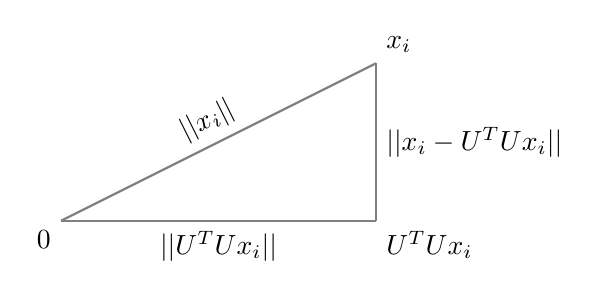
\begin{tikzpicture}[thick,draw=black!50, node distance=\layersep]
%https://tex.stackexchange.com/questions/96846/how-to-place-label-in-middle-of-line-above-and-below-with-tikz
    \tikzstyle{neuron}=[circle,fill=black!25,minimum size=17pt,inner sep=0pt, draw=black]
    \tikzstyle{input neuron}=[neuron, fill=green!50];
    \tikzstyle{output neuron}=[neuron, fill=red!50];
    \tikzstyle{hidden neuron}=[neuron, fill=blue!30];
    \tikzstyle{annot} = [text width=4em, text centered]

	\draw (0,0) --  node[below, pos=0.5] {$||U^TUx_i||$} ++  (4,0);
	\draw (4,0) --  node[right, pos=0.5] {$||x_i - U^TUx_i||$} ++  (0,2);
	\draw (4,2) --  (0,0)	node [midway, above, sloped] {$||x_i||$};

	\node [below left] at (0,0) {0};
	\node [below right] at (4,0) {$U^TUx_i$};
	\node [above right] at (4,2) {$x_i$};
\end{tikzpicture}
  \end{minipage}
  \vfill
\begin{minipage}[t][0.4\textheight][t]{\textwidth}
To see that the two conditions are equivalent, we will show that the variance in the data (which is fixed) is the sum of the \textbf{projected sample variance} and the \textbf{reconstruction error}.
\end{minipage}
\end{frame}


\begin{frame}<handout:0>[fragile]{Equivalence of Conditions}	
\begin{minipage}[t][0.4\textheight][t]{\textwidth}\centering
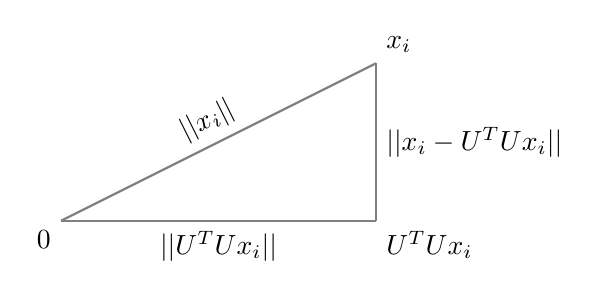
\begin{tikzpicture}[thick,draw=black!50, node distance=\layersep]
%https://tex.stackexchange.com/questions/96846/how-to-place-label-in-middle-of-line-above-and-below-with-tikz
    \tikzstyle{neuron}=[circle,fill=black!25,minimum size=17pt,inner sep=0pt, draw=black]
    \tikzstyle{input neuron}=[neuron, fill=green!50];
    \tikzstyle{output neuron}=[neuron, fill=red!50];
    \tikzstyle{hidden neuron}=[neuron, fill=blue!30];
    \tikzstyle{annot} = [text width=4em, text centered]

	\draw (0,0) --  node[below, pos=0.5] {$||U^TUx_i||$} ++  (4,0);
	\draw (4,0) --  node[right, pos=0.5] {$||x_i - U^TUx_i||$} ++  (0,2);
	\draw (4,2) --  (0,0)	node [midway, above, sloped] {$||x_i||$};

	\node [below left] at (0,0) {0};
	\node [below right] at (4,0) {$U^TUx_i$};
	\node [above right] at (4,2) {$x_i$};
\end{tikzpicture}
  \end{minipage}
  \vfill
\begin{minipage}[t][0.4\textheight][t]{\textwidth}
Taking the expectation of the Pythagorean decomposition 
$$
x_i = U^TUx_i + x_i - U^TUx_i
$$\pause
yields
$$
\widehat{E}\big[\,|| x_i ||^2\,\big] = \widehat{E}\big[\,|| U^TUx_i  ||^2\,\big] + \widehat{E}\big[\,|| x_i - U^TUx_i ||^2\,\big] 
$$
\end{minipage}
\end{frame}



\begin{frame}[fragile]{Equivalence of Conditions}
\begin{minipage}[t][0.4\textheight][t]{\textwidth}\centering
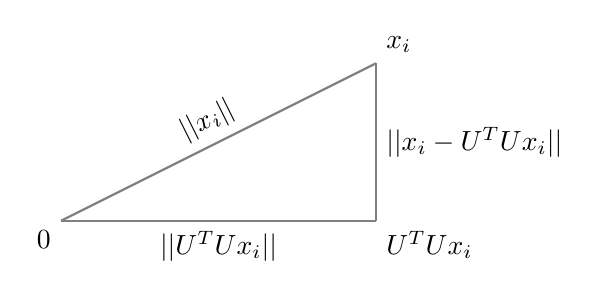
\begin{tikzpicture}[thick,draw=black!50, node distance=\layersep]
%https://tex.stackexchange.com/questions/96846/how-to-place-label-in-middle-of-line-above-and-below-with-tikz
    \tikzstyle{neuron}=[circle,fill=black!25,minimum size=17pt,inner sep=0pt, draw=black]
    \tikzstyle{input neuron}=[neuron, fill=green!50];
    \tikzstyle{output neuron}=[neuron, fill=red!50];
    \tikzstyle{hidden neuron}=[neuron, fill=blue!30];
    \tikzstyle{annot} = [text width=4em, text centered]

	\draw (0,0) --  node[below, pos=0.5] {$||U^TUx_i||$} ++  (4,0);
	\draw (4,0) --  node[right, pos=0.5] {$||x_i - U^TUx_i||$} ++  (0,2);
	\draw (4,2) --  (0,0)	node [midway, above, sloped] {$||x_i||$};

	\node [below left] at (0,0) {0};
	\node [below right] at (4,0) {$U^TUx_i$};
	\node [above right] at (4,2) {$x_i$};
\end{tikzpicture}
  \end{minipage}
  \vfill
\begin{minipage}[t][0.4\textheight][t]{\textwidth}
Taking the expectation of the Pythagorean decomposition 
$$
x_i = U^TUx_i + x_i - U^TUx_i
$$
yields
$$
\underset{\text{Sample Variance}}{\widehat{E}\big[\,|| x_i ||^2\,\big]} 
= 
\underset{\text{Projected Variance}}{\widehat{E}\big[\,|| U^TUx_i  ||^2\,\big]}
 + 
\underset{\text{Reconstruction Error}}{\widehat{E}\big[\,|| x_i - U^TUx_i ||^2\,\big]}
$$\pause
We see the minimizing reconstruction error is equivalent to maximizing projected variance. 
\end{minipage}
\end{frame}








\section{Principle Component Analysis}


\begin{frame}[fragile]{Principle Component Analysis}
The most common technique for factor analysis is \textbf{Principle Component Analysis} or \textbf{PCA}. It is in fact so common that "factor analysis" usually means "factor analysis that isn't PCA."\pause

PCA is a greedy algorithm with a beautiful mathematical interpretation. The idea is to proceed iteratively:\pause
\begin{itemize}
\item[] Find principle component (direction) that accounts for the largest possible variance.\pause
\item[] Project onto the subspace orthogonal to that vector.\pause
\item[] Repeat, collecting the orthogonal vectors into the rows of $U$ until $U$ is a $p\times p$ orthogonal matrix. 
\end{itemize}
\end{frame}



\begin{frame}[fragile]{Principle Component Analysis}
Let $x_i$ be demeaned data points and let $\bfX$ be the matrix whose rows are $x_i^T$. \pause We want to find a vector $w_{(1)} = (w_1,\ldots, w_p)_{(1)}$ with $||w_{(1)}|| = 1$ that maximizes the projected variance. Projection of $x_i$ onto $w_{(1)}$ is given by
$$
\textbf{proj}_{w_{(1)}} (x_i) = \frac{\langle x_1, w_{(1)}\rangle}{||w_{(1)}||^2}w_{(1)} = \langle x_1, w_{(1)}\rangle w_{(1)}\,.
$$\pause
Since $x_i$ have mean 0, the variance along $w_{(1)}$ is just 
$$
\widehat{E}\big[\,|| \langle x_1, w_{(1)}\rangle w_{(1)} ||^2\,\big] =\widehat{E}\big[\,\langle x_1, w_{(1)}\rangle^2\,\big]  \,.
$$\pause
Writing $\langle x_1, w_{(1)}\rangle = x_1\cdot w_{(1)}$ for the Cartesian inner product, our goal is to find
$$
w_{(1)} = \underset{||w_{(1)}||=1}{\text{argmax}}\left( \sum_{i=1}^N (x_i\cdot w_{(1)})^2  \right) 
= 
\underset{||w_{(1)}||=1}{\text{argmax}} \,\big(\,||\bfX w_{(1)}||^2\,\big)\,.
$$ 
\end{frame}




\begin{frame}[fragile]{Principle Component Analysis}
Writing the Euclidean norm as matrix multiplication, we see that it is equivalent to find
$$
w_{(1)} =
\underset{||w_{(1)}||=1}{\text{argmax}} \,\big(\,||\bfX w_{(1)}||^2\,\big)
=
\underset{||w_{(1)}||=1}{\text{argmax}} \,\big(\,w_{(1)}^T\bfX^T\bfX w_{(1)}\,\big)\,.
$$ \pause
The maximum is not so clear using our usual matrix differentiation. Indeed, the condition that $||w_{(1)}|| = 1$ plays an important role in the expression even having a maximum. We can use a Lagrangian procedure to rewrite the above as a single maximization problem:
$$
\mathcal{L} = w_{(1)}^T\bfX^T\bfX w_{(1)} + \lambda (1-w_{(1)}^Tw_{(1)} )\,.
$$
\textbf{(Question:)} What are the stationary points of $\mathcal{L} $?  \pause The solutions to the eigenvalue equation $\bfX^T\bfX w_{(1)}  = \lambda w_{(1)}$.


\end{frame}


\begin{frame}[fragile]{Principle Component Analysis}
Since the unit eigenvectors of $\bfX^T\bfX$ extremize $w_{(1)}^T\bfX^T\bfX w_{(1)}$, 
$$
\underset{||w_{(1)}||=1}{\text{argmax}} \,\big(\,w_{(1)}^T\bfX^T\bfX w_{(1)}\,\big)
$$\pause
is the eigenvector of $\bfX^T\bfX$ with the largest eigenvalue $\lambda$. \pause Furthermore,
$$
\widehat{\text{var}}(\mathbf{X}w_{(1)}) = \frac{1}{N}w_{(1)}^T\bfX^T\bfX w_{(1)} = \frac{1}{N}w_{(1)}^T\,(\lambda w_{(1)}) = \frac{\lambda}{N}\,.
$$\pause
But recall that the covariance matrix of the data
$$
\widehat{\text{Cov}}(\bfX) = \frac{1}{N} \bfX^T\bfX\,.
$$
We have shown that the first principle component is the eigenvector of the covariance matrix with the highest eigenvalue. 
\end{frame}




\begin{frame}[fragile]{Principle Component Analysis}
The result extends to the subsequent principle components. The proof proceeds identically to the proof for the first principle component and in fact constructs the orthogonal decomposition 
$$
\widehat{\text{Cov}}(\bfX)  = W\Lambda^{(p)}W^T\,,
$$
where $\lambda^{(p)} = \text{diag}(\lambda_1,\ldots, \lambda_p)$, with $\lambda_i>\lambda_{i+1}$.\pause

Computationally, the complexity is $O(Np^2 + p^3)$, the sum computing the covariance and eigenbasis respectively. 
\end{frame}



\begin{frame}[fragile]{Truncated Principle Component Analysis}
For dimensional reduction, we may stop this process at any step, revealing a \textbf{truncated} PCA matrix. Keeping only the first $k$ principle components yields a orthogonal matrix $W_{k}$ which projects $x_i$ to the space spanned by the first $k$ principle vectors. \pause 

Mathematically, this performs decomposition of the covariance matrix into 
$$
\widehat{\text{Cov}}(\bfX)  = W\Lambda^{(k)}W^T\,,
$$
where $\lambda^{(k)} = \text{diag}(\lambda_1,\ldots, \lambda_k)$, with $\lambda_i>\lambda_{i+1}$\,.
\end{frame}


\begin{frame}[fragile]{Machine Learning Examples: Iris Classification}
\includegraphics[width=10.8cm]{L14IrisClass.png}

\begin{tabular}{llcll}
\textbf{Sepal Length} & \textbf{Sepal Width} & \textbf{Petal Length} & \textbf{Petal Width} & \textbf{Species}\\ \hline
 	5.1 &	3.5 &	1.4 &	0.2 &	I. Setosa         \\ \hline
7.0 	& 3.2  &	4.7 &	1.4 &	I. Versicolor         \\ \hline
&&$\vdots$
\end{tabular}

Take as an example projection onto the first two principle component in the Iris data set from Lecture 1. 
\end{frame}


\begin{frame}[fragile]{Example: PCA for Iris}
  \begin{minipage}[t][0.7\textheight][t]{\textwidth}
	\centering \includegraphics[height=0.7\textheight]{L14Iris.png} 
  \end{minipage}
  \vfill
\begin{minipage}[t][0.3\textheight][t]{\textwidth}
There are four variables, with correlations given above. 
\end{minipage}
\end{frame}


\begin{frame}[fragile]{Example: PCA for Iris}
  \begin{minipage}[t][0.5\textheight][t]{\textwidth}
	\centering \includegraphics[height=0.5\textheight]{L14IrisPCA.png} 
  \end{minipage}
  \vfill
\begin{minipage}[t][0.5\textheight][t]{\textwidth}
Using PCA to project onto the first two principle components yields a projection onto 
$$
w_{(1)} = (0.36, -0.08,  0.86,  0.36)\,,\hspace{3em} w_{(2)} = (0.66,  0.73, -0.18 , -0.07)
$$\pause
We see the species are separable knowing only their features, and furthermore we have concrete measurement ratios to determine species.
\end{minipage}
\end{frame}





\begin{frame}[fragile]{Example: PCA for Iris}
  \begin{minipage}[t][0.5\textheight][t]{\textwidth}
	\centering \includegraphics[height=0.5\textheight]{L14IrisLDA.png} 
  \end{minipage}
  \vfill
\begin{minipage}[t][0.5\textheight][t]{\textwidth}
Compare for a moment with the LDA projection. LDA requires knowing the labels and requires significantly more computational time for a similar fit. 
\end{minipage}
\end{frame}




\begin{frame}[fragile]{Example: PCA MNIST}
  \begin{minipage}[t][0.5\textheight][t]{\textwidth}
	\centering \includegraphics[width=\textwidth]{L14MNISTPCA.png} 
  \end{minipage}
  \vfill
\begin{minipage}[t][0.5\textheight][t]{\textwidth}
The MNIST data set may provide one of the most startling examples. A simple PCA can be computed quite quickly and yields a wealth of information about the structure of the data set. 
\end{minipage}
\end{frame}


\begin{frame}[fragile]{Example: PCA MNIST}
  \begin{minipage}[t][0.5\textheight][t]{\textwidth}
	\centering \includegraphics[height=0.5\textheight]{L14MNISTPCA2.png} 
  \end{minipage}
  \vfill
\begin{minipage}[t][0.5\textheight][t]{\textwidth}
The MNIST data set may provide one of the most startling examples. A simple PCA can be computed quite quickly and yields a wealth of information about the structure of the data set. Projecting onto the first two components shows a lot of structure on the MNIST dataset. 
\end{minipage}
\end{frame}




\begin{frame}[fragile]{Example: PCA MNIST}
  \begin{minipage}[t][0.5\textheight][t]{\textwidth}
	\centering \includegraphics[width=\textwidth]{L14FMNISTPCA.png} 
  \end{minipage}
  \vfill
\begin{minipage}[t][0.5\textheight][t]{\textwidth}
This is not always as useful. Performing PCA on the fashion MNIST data set doesn't yield as strong of forms as on the digits MNIST. On the other hand, we see much more structure and organization in the projection onto eignevectors. 
\end{minipage}
\end{frame}



\begin{frame}[fragile]{Example: PCA MNIST}
  \begin{minipage}[t][0.5\textheight][t]{\textwidth}
	\centering \includegraphics[height=0.5\textheight]{L14FMNISTPCA2.png} 
  \end{minipage}
  \vfill
\begin{minipage}[t][0.5\textheight][t]{\textwidth}
This is probably because the MNIST dataset lies ``close'' to a linear subspace representation, while the Fashion MNIST dataset lies on a curved manifold. 

For an excellent article on visualization of MNIST, see \url{http://colah.github.io/posts/2014-10-Visualizing-MNIST/}
\end{minipage}
\end{frame}







\begin{frame}[fragile]{Nonlinear PCA}
  \begin{minipage}[t][0.5\textheight][t]{\textwidth}
	\centering \includegraphics[height=0.5\textheight]{L5PCAStudent.png} 
  \end{minipage}
  \vfill
\begin{minipage}[t][0.5\textheight][t]{\textwidth}
In the context of regression, PCA can perform subset selection for us. In the graph above, we used PCA to project the features of the Student Admission dataset onto the first two principle components. It's important to note though that PCA doesn't know anything about the labels $Y$. This can be an advantage, unlabeled data can import the PCA (an unlabeled data is often cheap).
\end{minipage}
\end{frame}



\begin{frame}[fragile]{Nonlinear PCA}
  \begin{minipage}[t][0.7\textheight][t]{\textwidth}
	\centering \includegraphics[height=0.7\textheight]{L5PCAStudent2.png} 
  \end{minipage}
  \vfill
\begin{minipage}[t][0.3\textheight][t]{\textwidth}
But that doesn't necessarily lead to a better fit.
\end{minipage}
\end{frame}




\section{Nonlinear PCA}

\begin{frame}[fragile]{Nonlinear PCA}
  \begin{minipage}[t][0.5\textheight][t]{\textwidth}
	\centering \includegraphics[height=0.5\textheight]{L14KernelPCA.png} 
  \end{minipage}
  \vfill
\begin{minipage}[t][0.5\textheight][t]{\textwidth}
Of course, linear methods may be almost useless if the underlying structure isn't linear. For truly unknown structure we must construct smoothing maps using splines, random graphs, or other high complexity techniques. \pause For example, in the distribution above linear PCA will do nothing to reduce the complexity of the data set. 
\end{minipage}
\end{frame}


\begin{frame}[fragile]{Nonlinear PCA}
  \begin{minipage}[t][0.5\textheight][t]{\textwidth}
	\centering \includegraphics[height=0.5\textheight]{L14KernelPCA.png} 
  \end{minipage}
  \vfill
\begin{minipage}[t][0.5\textheight][t]{\textwidth}
However, whenever we have linear methods there is the hope that we can apply the linear methods to generated features and get a a better fit. For nonlinear PCA, this means that we generate a high dimensional feature space, say $(1,X,X^2)$, and then project down onto a low dimensional subspace of this feature set, that is a normalized polynomial feature. 
\end{minipage}
\end{frame}


\begin{frame}[fragile]{Nonlinear PCA}
In keeping with the literature, let $\phi:\mathcal{X}\to \widetilde{\mathcal{X}}$ be an embedding of the feature space into a higher dimensional space (say, the space of degree $d$ polynomials in the features). \pause Assume that projection has 0 mean. \pause

The covariance matrix in the embedded space can be written
$$
\widetilde{C} = \widetilde{\text{Cov}} = \frac{1}{N}\sum_{i=1}^N\phi(x_i)\phi(x_i)^T\,,
$$\pause
where $\tilde{C}$ has eigenvectors $w_k$ and eigenvalues $\widetilde{C}w_k = \lambda_kw_k$. 
\end{frame}



\begin{frame}[fragile]{Nonlinear PCA}
Since 
$$
\widetilde{C}w_k = \frac{1}{N}\sum_{i=1}^N\phi(x_i)\big(\,\phi(x_i)^T\,w_k\big) = \lambda_kw_k\,,
$$\pause
we can write
$$
w_k = \sum_{i=1}^N a_{ki}\phi(x_i)\,,\,\,\,\text{where}\,\,\, a_{ki} = \frac{1}{N}\,\phi(x_i)^T\,w_k\,.
$$\pause
Notice that this projection doesn't depend on knowing $\phi$, but only the inner product $K(x_i,x_j) = \phi(x_i)^T\phi(x_j)$. We can write
$$
\phi(x_\ell)^T\frac{1}{N}\sum_{i=1}^N\phi(x_i)\big(\,\phi(x_i)^T\,\sum_{j=1}^N a_{kj}\phi(x_j)\big) = \lambda_k\phi(x_\ell)^T\sum_{j=1}^N a_{kj}\phi(x_j)\,,
$$\pause
or
$$
\frac{1}{N}\sum_{i=1}^NK(x_\ell, x_i)\sum_{i=j}^N K(x_i, x_j) = \lambda_k\sum_{j=1}^N K(x_\ell, x_j)\,.
$$
\end{frame}



\begin{frame}[fragile]{Nonlinear PCA}
Since 
$$
\widetilde{C}w_k = \frac{1}{N}\sum_{i=1}^N\phi(x_i)\big(\,\phi(x_i)^T\,w_k\big) = \lambda_kw_k\,,
$$\pause
we can write
$$
w_k = \sum_{i=1}^N a_{ki}\phi(x_i)\,,\,\,\,\text{where}\,\,\, a_{ki} = \frac{1}{N}\,\phi(x_i)^T\,w_k\,.
$$\pause
If $K(x_i,x_j) = \phi(x_i)^T\phi(x_j)$ is simply computable, then for any $\phi(x_\ell)^T$ the first equation can be written
$$
\phi(x_\ell)^T\frac{1}{N}\sum_{i=1}^N\phi(x_i)\big(\,\phi(x_i)^T\,\sum_{j=1}^N a_{kj}\phi(x_j)\big) = \lambda_k\phi(x_\ell)^T\sum_{j=1}^N a_{kj}\phi(x_j)\,,
$$\pause
or
$$
\frac{1}{N}\sum_{i=1}^NK(x_\ell, x_i)\sum_{i=j}^N K(x_i, x_j) = \lambda_k\sum_{j=1}^N K(x_\ell, x_j)\,.
$$
\end{frame}





\begin{frame}[fragile]{Nonlinear PCA}
Writing $\mathbf{K}_{ij} = K(x_i,x_j)$, and $a_k = [a_{k1},\ldots, a_{kN}]^T$ \pause
$$
\frac{1}{N}\sum_{i=1}^NK(x_\ell, x_i)\sum_{i=j}^N K(x_i, x_j) = \lambda_k\sum_{j=1}^N K(x_\ell, x_j)\,,
$$
can be written
$$
\mathbf{K}^2a_k = \lambda_kN\mathbf{K}a_k\,.
$$\pause
So the higher dimensional fitting is solved by the kernel eigenvalue problem
$$
\mathbf{K}a_k = \lambda_kNa_k\,.
$$\pause
Again, this trick is restricted to transformations for which there exists a computable kernel, but if one exists this is a remarkable reduction in complexity. 
\end{frame}


\begin{frame}[fragile]{Kernels}
In the computation above $K(X,X')$ is called a \textbf{kernel}
$$
K(X,X') = \langle \phi(X),\phi X')\rangle\,.
$$\pause
For example, for degree 2 polynomials $\phi(X) = 1 + X + X^2$, which we may write as a feature transform
$$
\phi:X \mapsto (1,X,X^2)\,.
$$\pause
The inner product $\phi(X)^T\phi(X')$  is 
$$
\phi(X)^T\phi(X') = 1 + XX' + X^2(X')^2 = (1 + \langle X, X'\rangle)^2 = K(X,X')\,.
$$
Note that the kernel $K(X,X')$ is computed in the domain, not in the transformed space and so is much easier to evaluate. Lets see a slightly more complex example. 
\end{frame}




\begin{frame}[fragile]{Kernels}
Assume that $X$ has two features $X_1$ and $X_2$ and we want to perform PCA on the quadratic combination of those features:
$$\phi(X) = (1,\sqrt2 X_1,\sqrt2X_2, X_1^2,X_2^2,\sqrt2X_1X_2)\,.$$
Here, the features have been normalized for ease of computation but need not be.\pause

For nonliner PCA, we need to compute
$$
\phi(X)^T\phi(X') = 1 + 2X_1X_1' + 2X_2X_2' + (X_1X_1')^2 + (X_2X_2')^2 + 2(X_1X_1'X_2X_2')\,.
$$
Notice, this takes the same form as before:
\begin{align*}
K(X,X') &= (1+\langle X,X'\rangle)^2
\\
K(X,X') &= (1+X_1X_1' + X_2X_2')^2
\\
K(X,X') &= 1 + 2X_1X_1' + 2X_2X_2' + (X_1X_1')^2 + (X_2X_2')^2 + 2(X_1X_1'X_2X_2')
\end{align*}
\end{frame}


\begin{frame}[fragile]{Kernels}
If the kernel is easy to compute, we can do nonlinear PCA. Three popular choices for transformations with kernels are
\begin{table}[]
\begin{tabular}{ll}
\hline
Degree $d$ Polynomials               & $K(X,X') = (1+\langle X,X'\rangle)^d$                                                  
 \\ \hline
Radial Basis &  $K(X,X') = \exp\big(-\gamma||X-X'||^2\big)$                      
\\ \hline
Neural Networks                    & $K(X,X') =\tanh(w\langle X,X'\rangle + b)$ \\ \hline
\end{tabular}
\end{table}\pause
You will notice that these are much easier to compute than having to map $X$ forward to a high dimensional feature space and then compute the inner project there.
\end{frame}




\begin{frame}[fragile]{Nonlinear PCA}
  \begin{minipage}[t][0.5\textheight][t]{\textwidth}
	\centering \includegraphics[height=0.5\textheight]{L14KernelPCA.png} 
  \end{minipage}
  \vfill
\begin{minipage}[t][0.5\textheight][t]{\textwidth}
Applying the radial basis function kernel PCA to the concentric circle data set results in a dramatic clustering.
\end{minipage}
\end{frame}


\begin{frame}[fragile]{Nonlinear PCA}
  \begin{minipage}[t][0.5\textheight][t]{\textwidth}
	\centering \includegraphics[height=0.5\textheight]{L14KernelPCA2.png} 
  \end{minipage}
  \vfill
\begin{minipage}[t][0.5\textheight][t]{\textwidth}
Applying the radial basis function kernel PCA to the concentric circle data set results in a dramatic clustering.
\end{minipage}
\end{frame}





\begin{frame}[fragile]{References}
References for this lecture: BS, Chapters 15, 16, 18 and ESII, Chapters 9, 12.  

Charles Minard's Map:
\url{https://en.wikipedia.org/wiki/Charles_Joseph_Minard}
\end{frame}


\end{document}

%%%%%%%%%%%%%%%%%%%%%%%%%%%%%%%%%%
%
% |   __|___ _| |  |    \ ___ ___ _ _ _____ ___ ___| |_ 
% |   __|   | . |  |  |  | . |  _| | |     | -_|   |  _|
% |_____|_|_|___|  |____/|___|___|___|_|_|_|___|_|_|_|                                                   
%
%%%%%%%%%%%%%%%%%%%%%%%%%%%%%%%%%%



%%%%%%%%%%%%%%%%%%%%%%%%%%%%%%%%%%%%%%%%%%%
%%%%%%%%%%%%%%%%%%%%%%%%%%%%%%%%%%%%%%%%%%%
%%%%%%%%%%%%%%%%%%%%%%%%%%%%%%%%%%%%%%%%%%%



\begin{frame}[fragile]{Introduction}

\end{frame}




\begin{frame}[fragile]{Binary Classification}
  \begin{minipage}[t][0.5\textheight][t]{\textwidth}
	\centering \includegraphics[height=0.5\textheight]{.png} 
  \end{minipage}
  \vfill
\begin{minipage}[t][0.5\textheight][t]{\textwidth}

\end{minipage}
\end{frame}



\begin{frame}[fragile]{Test}
\begin{minipage}[t][0.5\textheight][t]{\textwidth}\centering
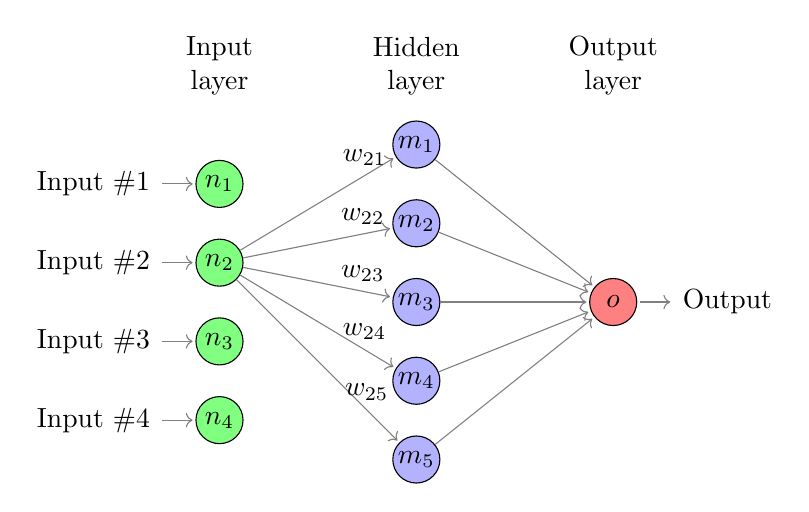
\begin{tikzpicture}[shorten >=1pt,->,draw=black!50, node distance=\layersep]
%https://tex.stackexchange.com/questions/96846/how-to-place-label-in-middle-of-line-above-and-below-with-tikz
    \tikzstyle{every pin edge}=[<-,shorten <=1pt]
    \tikzstyle{neuron}=[circle,fill=black!25,minimum size=17pt,inner sep=0pt, draw=black]
    \tikzstyle{input neuron}=[neuron, fill=green!50];
    \tikzstyle{output neuron}=[neuron, fill=red!50];
    \tikzstyle{hidden neuron}=[neuron, fill=blue!30];
    \tikzstyle{annot} = [text width=4em, text centered]

    % Draw the input layer nodes
    \foreach \name / \y in {1,...,4}
    % This is the same as writing \foreach \name / \y in {1/1,2/2,3/3,4/4}
        \node[input neuron, pin=left:Input \#\y] (I-\name) at (0,-\y) {$n_\y$};

    % Draw the hidden layer nodes
    \foreach \name / \y in {1,...,5}
        \path[yshift=0.5cm]
            node[hidden neuron] (H-\name) at (\layersep,-\y cm) {$m_\y$};

    % Draw the output layer node
    \node[output neuron,pin={[pin edge={->}]right:Output}, right of=H-3] (O) {$o$};

    % Connect every node in the input layer with every node in the
    % hidden layer.
%    \foreach \source in {1,...,4}
%        \foreach \dest in {1,...,5}
%            \draw (I-\source) -- node[below] {$w_ij$} ++ (H-\dest);


%    \foreach \source in {1,...,4}
        \foreach \dest in {1,...,5}
            \draw (I-2) -- node[above, pos=0.8] {$w_{2\dest}$} ++ (H-\dest);

    % Connect every node in the hidden layer with the output layer
    \foreach \source in {1,...,5}
        \path (H-\source) edge (O);

    % Annotate the layers
    \node[annot,above of=H-1, node distance=1cm] (hl) {Hidden layer};
    \node[annot,left of=hl] {Input layer};
    \node[annot,right of=hl] {Output layer};
\end{tikzpicture}
  \end{minipage}
  \vfill
\begin{minipage}[t][0.5\textheight][t]{\textwidth}

\end{minipage}


\end{frame}




\begin{frame}[fragile]{Point Variance of Linear Predictor}

\begin{align*}
\action<+->{ &=&&}
\\
\action<+->{  &=   && }
\end{align*}
\action<+->{The}
\end{frame}



\begin{frame}[fragile]{Correlation}
\begin{itemize}
\item[] \textbf{Serial No.} is basically uncorrelated with anything. \pause
\item[] \textbf{Admit} is highly correlated with \textbf{CGPA}, \textbf{TOEFL Score} and \textbf{GRE Score}\pause
\item[] \textbf{Research} has a lowish correlation with \textbf{Admit}, but also with everything else.  
\end{itemize}
\end{frame}











\begin{frame}[fragile]{Bias, Variance and Parameters}
  \begin{minipage}[t][0.5\textheight][t]{\textwidth}
	\centering
	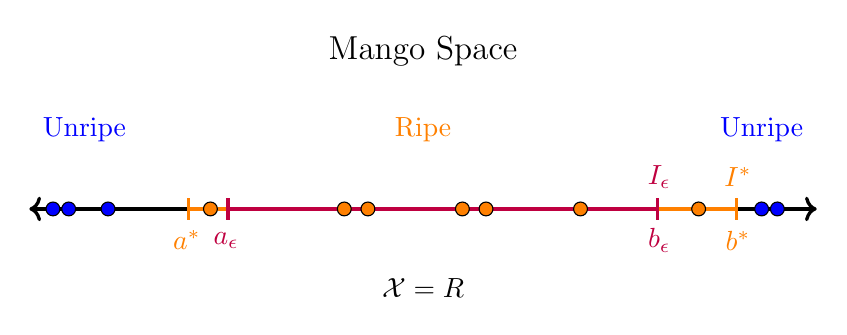
\begin{tikzpicture}
		\draw[<->,very thick] (-5,0) -- (5,0);
		\draw[color = orange, |-|,very thick] (-3,0) -- (4,0);
		\node[color=orange] at (4,.4) {$I^*$};
		\node at (0,2) {\large Mango Space} ;
		\node at (0,-1) {$\mathcal{X} = \mathbb{R}$} ;
		\node [color=blue] at (-4.3,1) {Unripe} ;
		\node [color=blue] at (4.3,1) {Unripe} ;
		\node [color=orange] at (0,1) {Ripe} ;

		\node [color=orange] at (-3,-.4) {$a^*$} ;
		\node [color=orange] at (4,-.4) {$b^*$} ;

		\draw [color=purple, |-|,very thick] (-2.5,0) -- (3,0);
		\node [color=purple] at (3,.4) {$I_\epsilon$} ;
		\node [color=purple] at (-2.5,-.4) {$a_\epsilon$} ;
		\node [color=purple] at (3,-.4) {$b_\epsilon$} ;

%		\draw [color=olive, |-|,very thick] (-3.5,0) -- (2.5,0);
%		\node [color=olive] at (3,.4) {$h_{\mathcal{T}}$} ;



		\node[circle,draw=black, fill=orange, inner sep=0pt,minimum size=5pt] at (2,0) {};
		\node[circle,draw=black, fill=orange, inner sep=0pt,minimum size=5pt] at (-1,0) {};
		\node[circle,draw=black, fill=orange, inner sep=0pt,minimum size=5pt] at (-.7,0) {};
		\node[circle,draw=black, fill=orange, inner sep=0pt,minimum size=5pt] at (.5,0) {};
		\node[circle,draw=black, fill=orange, inner sep=0pt,minimum size=5pt] at (.8,0) {};
		\node[circle,draw=black, fill=orange, inner sep=0pt,minimum size=5pt] at (-2.7,0) {};
		\node[circle,draw=black, fill=orange, inner sep=0pt,minimum size=5pt] at (3.5,0) {};

		\node[circle,draw=black, fill=blue, inner sep=0pt,minimum size=5pt] at (-4.5,0) {};
		\node[circle,draw=black, fill=blue, inner sep=0pt,minimum size=5pt] at (-4,0) {};
		\node[circle,draw=black, fill=blue, inner sep=0pt,minimum size=5pt] at (-4.7,0) {};
		\node[circle,draw=black, fill=blue, inner sep=0pt,minimum size=5pt] at (4.3,0) {};
		\node[circle,draw=black, fill=blue, inner sep=0pt,minimum size=5pt] at (4.5,0) {};
	\end{tikzpicture}
  \end{minipage}
  \vfill
  \begin{minipage}[t][0.5\textheight][t]{\textwidth}
Lets understand this visually.
$$
Err(x_0) = \sigma_\epsilon^2 + [E_\cT[\hat f(x_0)] - f(x_0)]^2 + E_\cT\big[ \hat{f}(x_0) - E_\cT[\hat{f}(x_0)] \big]^2\,.
$$\pause
Consider a data set, 
\end{minipage}
\end{frame}





























